\chapter{DIODE CHARACTERISTICS}

\subsection*{AIM}
\paragraph{}To design and implement a circuit for simulating the V-I characteristics of a diode.

\subsection*{DESIGN AND CIRCUIT DIAGRAM}
\paragraph{}

Inorder to draw the diode characteristics, we have to use a DC source of voltage which may be varied during simulation. The diode in the circuit should be associated with a coresponding `Diode model' during  simulations. As in a hardware circuits lab, a curernt limiting resistor may also be used in series with the diode and the DC source. The resulting circuit diagram is shown in the Figure \ref{diodeckt}  below:
\begin{figure}[h]
\centering
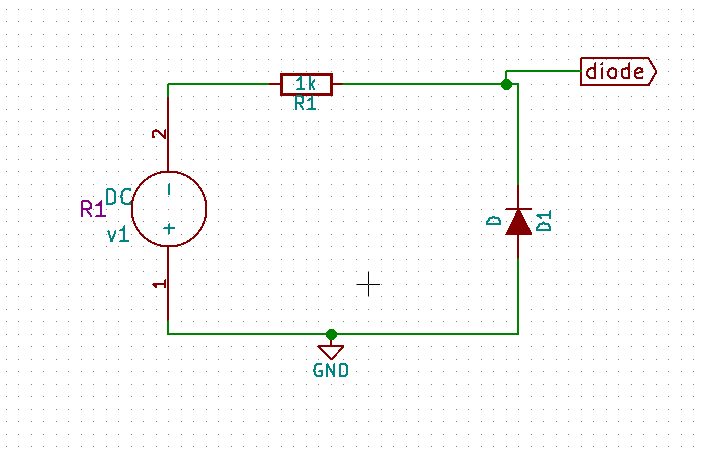
\includegraphics[width=0.8\textwidth]{diodeckt.png}
\caption{Schematic diagram for diode characteristics}
\label{diodeckt}
\end{figure}

\subsection*{PROCEDURE}

\subsubsection{Launch eSim}

\paragraph{}
 Launching eSim will take you to the dialog box which asks for the default workspace. Browsw the folders and set the wokspace location. It will finally end up in the eSim window shown in Figure \ref{LaunchWindow}.
\begin{figure}[h]
\centering
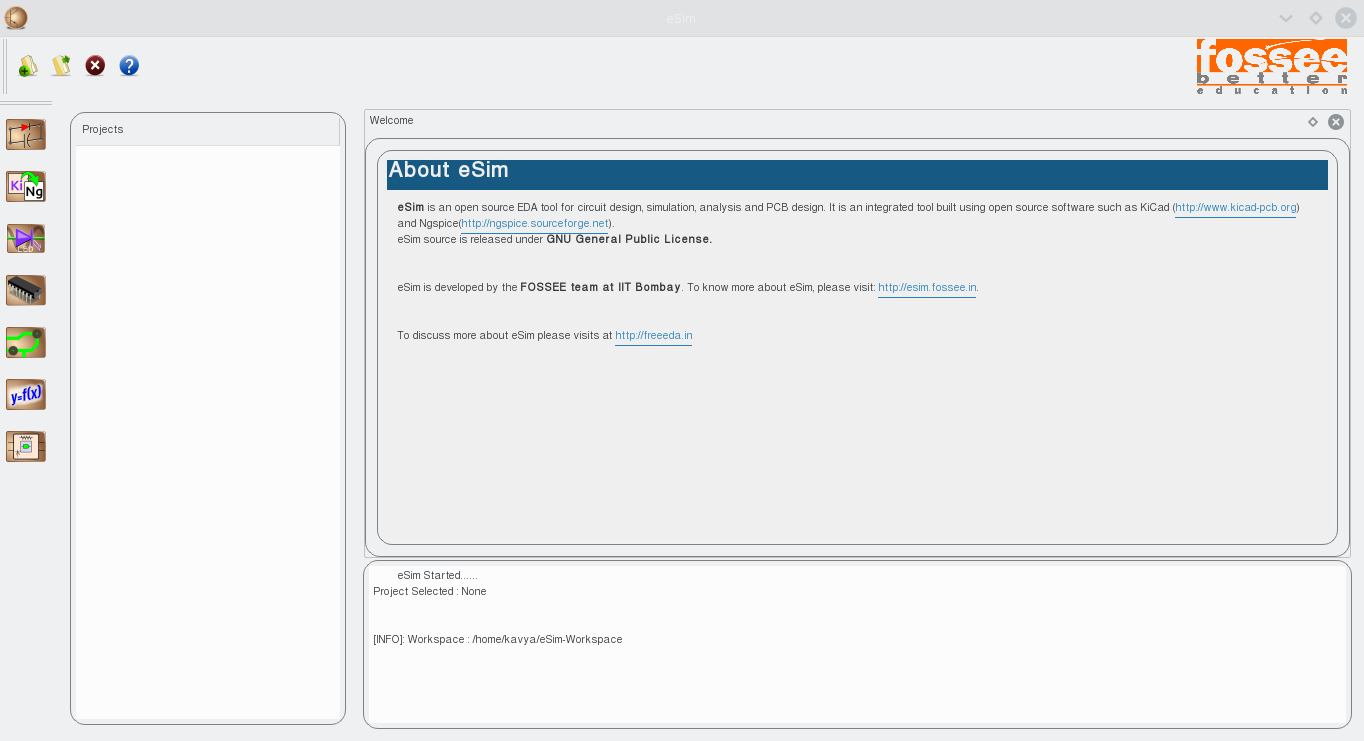
\includegraphics[width=0.8\textwidth]{LaunchWindow.png}
\caption{Launching eSim will take you to this window}
\label{LaunchWindow}
\end{figure}

\subsubsection{Create a New Project}

\paragraph{ } The new project is created by clicking the New icon on the
menubar. The name of the project is given in the pop up window as shown in Figure.\ref{newproject}.
\begin{figure}[h]
\centering
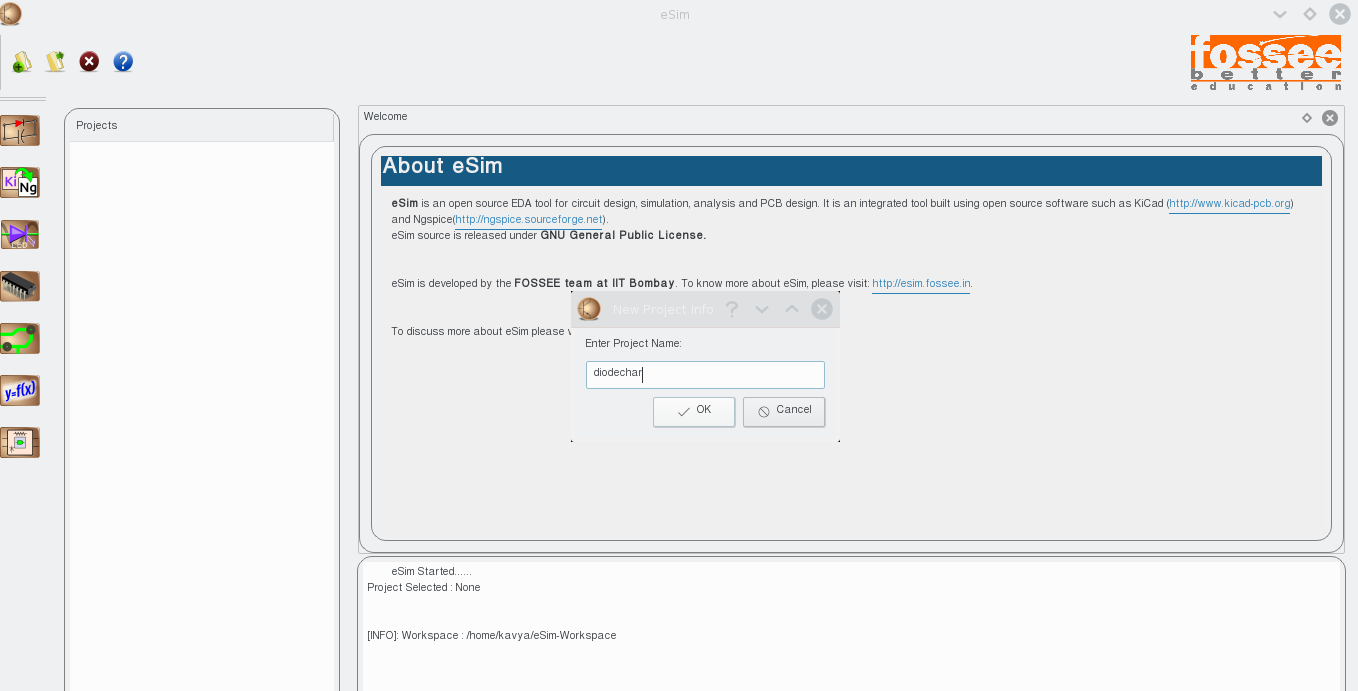
\includegraphics[width=\textwidth]{newproject.png}
\caption{Creating new project}
\label{newproject}
\end{figure}

\subsubsection{Create the Schematic}

\paragraph{}  To create the schematic, click the very first icon of the
left toolbar as shown in the Figure \ref{newschematic} .This will open KiCad Eeschema.


\begin{figure}[h]
\centering
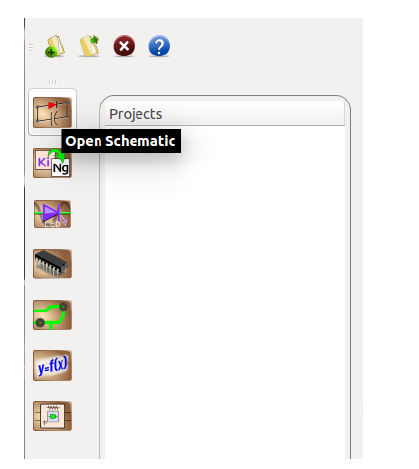
\includegraphics[width=0.5\textwidth, height=6cm]{newschematic.png}
\caption{Creating new schematic diagram}
\label{newschematic}
\end{figure}

To create a schematic in KiCad, we need to place the required components. See Figure \ref{kicad}

\begin{figure}[h]
\centering
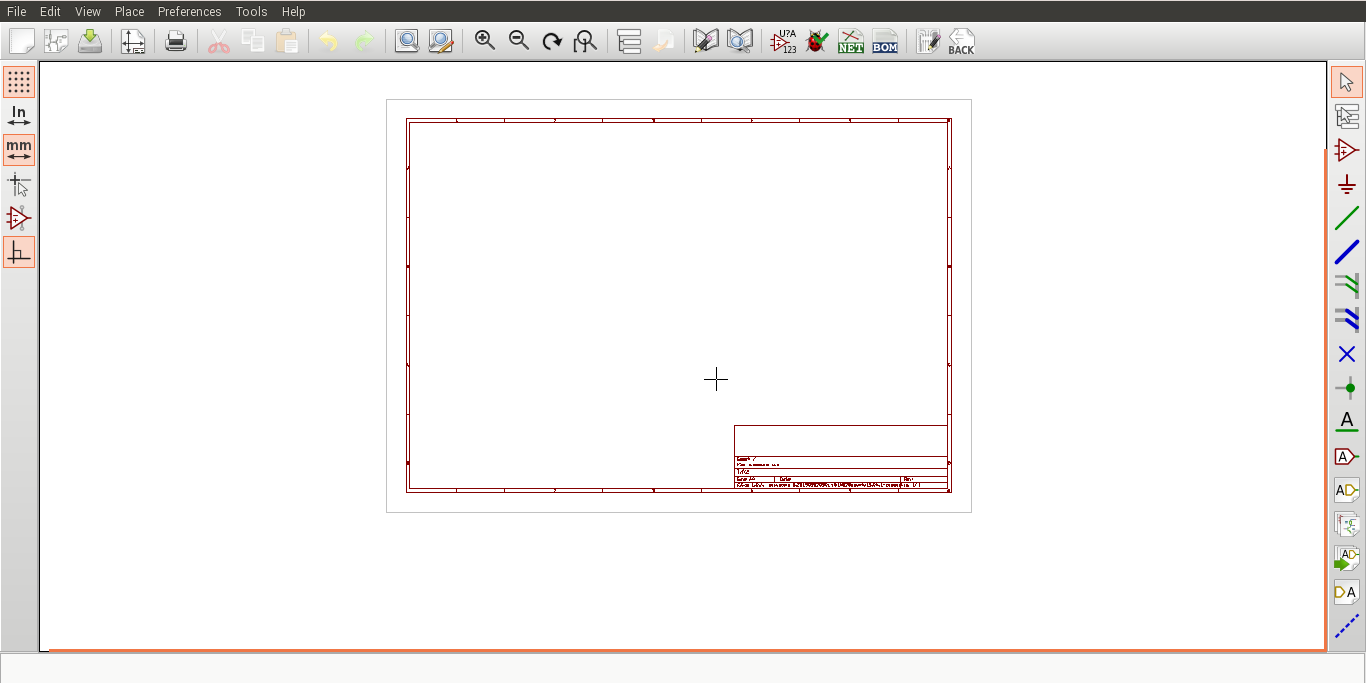
\includegraphics[width=0.5\textwidth, height=6cm]{kicad.png}
\caption{The Kicad Eeschema page}
\label{kicad}
\end{figure}

 Figure \ref{placecomponent}
shows the icon on the right toolbar which opens the component library. After all the required components of the simple RC circuit are placed, wiring is
done using the Place Wire option as shown in the Figure \ref{placewire}.Scroll up and down for zooming in and out.


\begin{figure}
\begin{minipage}{.5\textwidth}
  \centering
  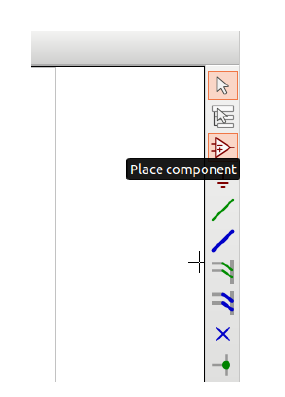
\includegraphics[width=\linewidth]{placecomponent.png}
  \caption{Place component icon}
  \label{placecomponent}
\end{minipage}%
\begin{minipage}{.5\textwidth}
  \centering
  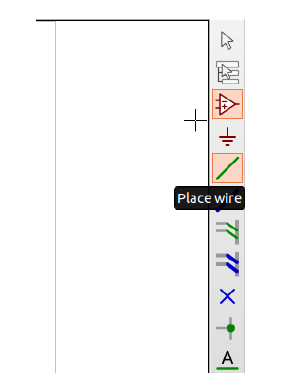
\includegraphics[width=\linewidth]{placewire.png}
  \caption{Place wire icon}
  \label{placewire}
\end{minipage}
\end{figure}


\paragraph{Placing the Components:} Normally all the components availbale in eSim can be chosen by left mouse click in the grid. The components are listed in different libraries. See Figure \ref{librarylist}.

\begin{figure}[h]
\centering
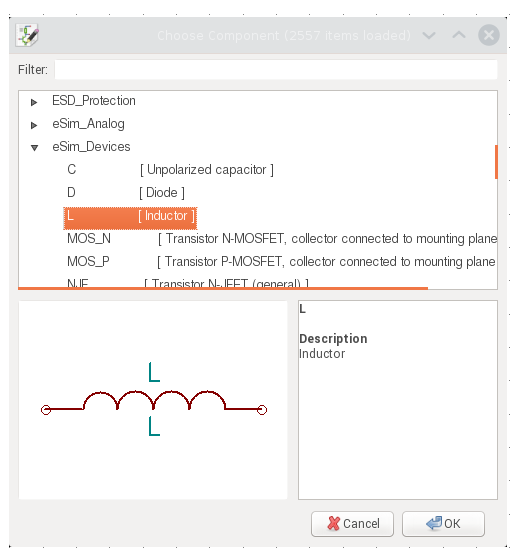
\includegraphics[width=0.5\textwidth, height=4cm]{librarylist.png}
\caption{The Kicad Libraries of components}
\label{librarylist}
\end{figure}

\begin{itemize}
\item
Choose DC source from eSim\_Sources
\item
Choose R from eSim\_Devices
\item
Choose D from eSim\_Devices
\item
Choose GND from power
\end{itemize}

Select the resistor and edit its component value to 1k as shown in Figure \ref{editvalue}.

\begin{figure}[h]
\centering
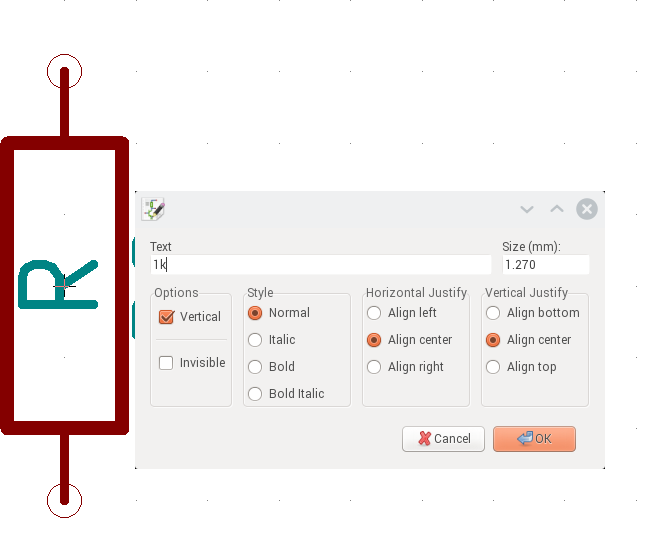
\includegraphics[width=0.5\textwidth, height=6cm]{editvalue.png}
\caption{Editing the value field of component R}
\label{editvalue}
\end{figure}

Wire the components to get the circuit. A global label `diode' has been added to identify that node whose voltage will be later recorded and plotted.

\paragraph{Annotating the circuit:} Once the schematic diagram is completed, annotate it so that the `question marks' associated with the components are converted to meaningful numbers automatically.For that choose annotate button from the top toolbar(See Figure \ref{toptoolbar} and in the subsequenct dialogue boxes appearing click ok and finally close. See Figure \ref{annotation}.

\begin{figure}[h]
\centering
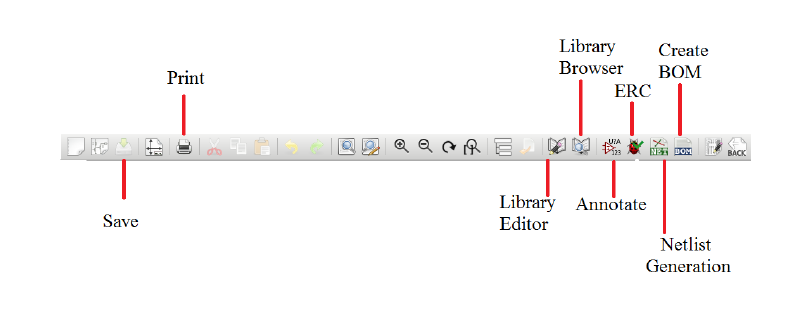
\includegraphics[width=\textwidth, height=4cm]{toptoolbar.png}
\caption{Choose annotate from the toop tool bar}
\label{toptoolbar}
\end{figure}



Now we have the circuit diagram as shown in Figure \ref{diodeckt}.


\paragraph{Note:} If some libraries are found missing, you can add them from the `Preferences` menu by following the procedure: 

\begin{enumerate}
\item
Choose `Component Libraries' from Preferences menu.

\item
Click on the Add button on the top right side of the window.

\item
Choose the required libraries from `user/share/kicad/library' and click OK button

\end{enumerate}

\subsubsection{Create Netlist}

\paragraph{}To simulate the circuit that has been created in the previous section, we need to generate
its netlist. Netlist is a list of components in the schematic along with their connection
information. To do so, click on the Generate netlist tool from the top toolbar. Click on
spice from the window that opens up. Check the option Default Format. Then click
on Generate. This is shown in Fig. 5.15. Save the netlist. This will be a .cir file. Do
not change the directory while saving.See Figure \ref{createnetlist}.
 Now the netlist is ready to be simulated. 
\begin{figure}
\begin{minipage}{.5\textwidth}
  \centering
  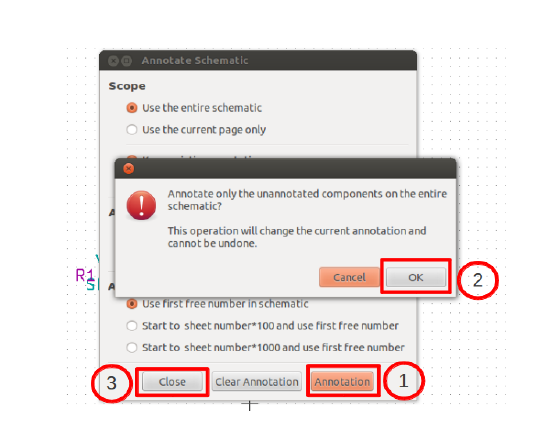
\includegraphics[width=\linewidth]{annotation.png}
  \caption{Annotation}
  \label{annotation}
\end{minipage}%
\begin{minipage}{.5\textwidth}
  \centering
  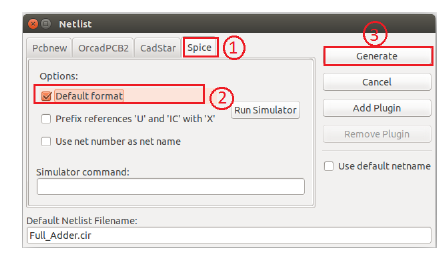
\includegraphics[width=\linewidth]{createnetlist.png}
  \caption{Netlist Generation}
  \label{createnetlist}
\end{minipage}
\end{figure}

\subsubsection{KiCad to Ngspice conversion}

\paragraph{} To convert KiCad netlist of RC circuit to NgSpice
compatible netlist click on KiCad to Ngspice icon as shown in Figure \ref{kcd2spice}.  Now you can choose the type of analysis, source details, device models ngspice models and subcircuit models.


\begin{figure}[h]
\centering
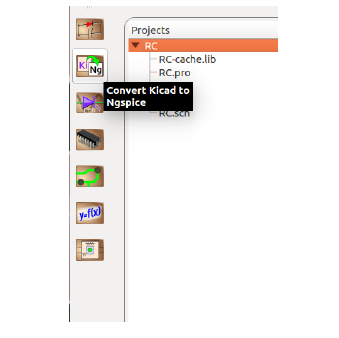
\includegraphics[width=0.5\textwidth, height=4cm]{kcd2spice.png}
\caption{Choose Kicad to Ngspice tool}
\label{kcd2spice}
\end{figure}


\paragraph{Analysis:}Choose DC analysis type. Give the values of DC variables as shown in Figure \ref{analysis}. Enter the name of your DC source as on the circuit (here v1) and let its value be varied from -15V to +15V with a step of 0.1 V.

\begin{figure}[h]
\centering
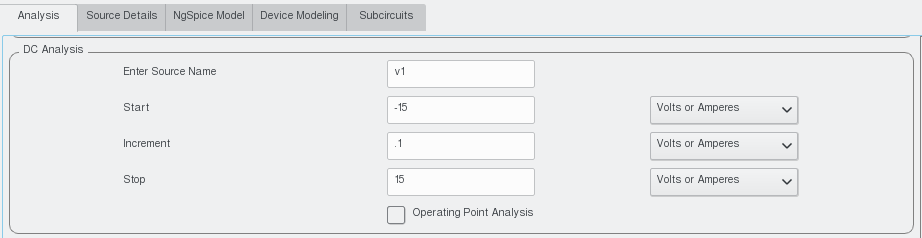
\includegraphics[width=\textwidth, height=4cm]{analysis.png}
\caption{Choose DC analysis type and enter the values}
\label{analysis}
\end{figure}

\paragraph{Source Details:} Leave this empty.

\paragraph{Ngspice Model:} No Ngspice model to be given.

\paragraph{Device Model:} The Diode is a device whose model details must be given for simulation. Let us choose the generic diode model availabe in the eSim model library. Browse it from /opt/eSim/src/deviceModelLibrary/Diode/D.lib. See Figure \ref{diodemodel}.
\begin{figure}[h]
\centering
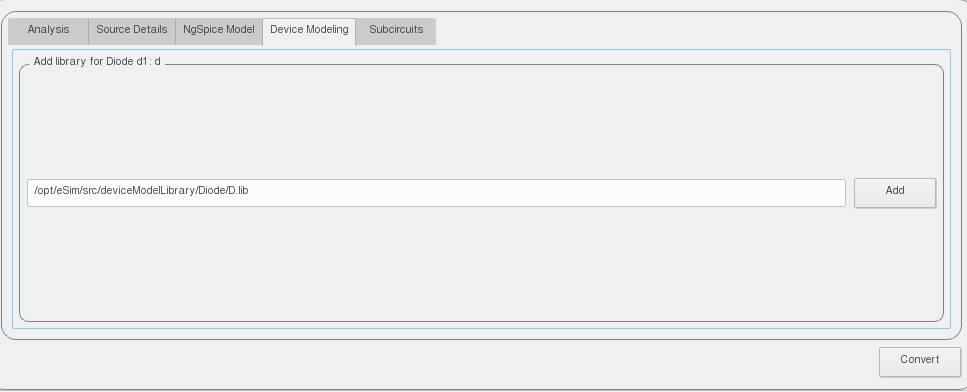
\includegraphics[width=\textwidth, height=6cm]{diodemodel.png}
\caption{Choose the required diode model}
\label{diodemodel}
\end{figure}

\paragraph{Subcircuits:} No subcircuits to be given.

\noindent Once these details are provided click on convert button. See Figure \ref{diodemodel}. Now you are ready to see the simulation results.

\subsubsection{Simulate} To run Ngspice simulation click the simulation icon in the left tool bar. It will open up two windows - ngspice plotting window and python plotting window. Inorder to plot the diode characteristics let us use the commands in ngspice plotting window. 

\paragraph{}We need to plot the value of voltage across the diode Vs the current through it. Since the current through the diode is same as the current through the voltage source,v1 (since both are in series connection) let us use the command:

\texttt{plot i(v1) vs v(diode)}

This would pop up the required characteristics fo the diode as defined in the diode model D.lib. For a differnt diode model the characteristics would be slightly different.

The resultant characteristics is shown in the Figure \ref{diodechara}.

\begin{figure}[h]
\centering
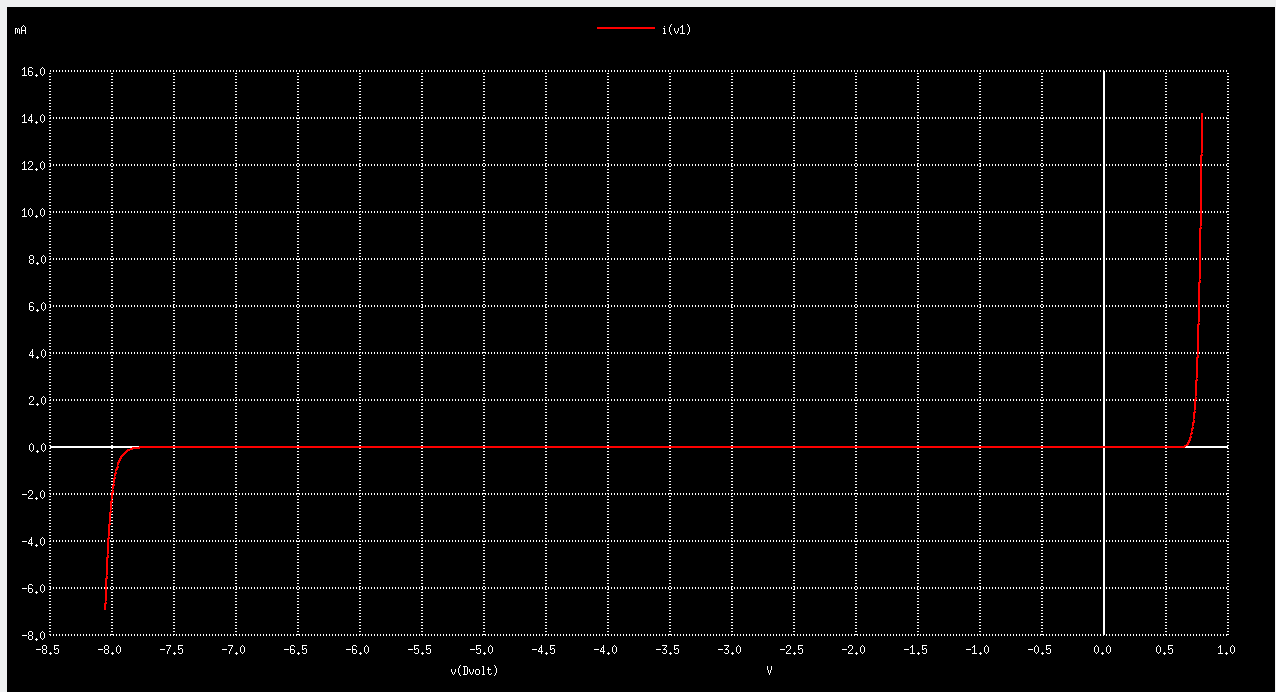
\includegraphics[width=12cm, height=6cm]{diodechar.png}
\caption{The characteristics of Diode}
\label{diodechara}
\end{figure}

\section*{RESULT}
The circuit for plotting the charateristics of diode was implemented and simulated.


